\chapter{Conclusions \& Musings}
\clearpage

%%%%%%%%%% TRADITIONAL CONCLUSIONS %%%%%%%%%%  
Vascular malformations are a class of lesion that are both phenotypically and genetically heterogeneous. Despite this heterogeneity, they share an overarching pathogenic mechanism whereby the initial formation of a lesion is seeded by a somatic mutation. These mutations may be in genes involved in canonical vascular development and maintenance or may be in well characterized oncogenes; nonetheless, somatic mutations play an integral role in the pathogenesis of many---if not all---vascular malformations. The studies described herein were performed with the goal of broadening our understanding of how somatic mutations may contribute to the pathogenesis of vascular malformations. Specifically, I aimed to show that somatic mutations may drive three distinct phases in the pathogenesis of vascular malformations: initiation (Chapter 2), progression (Chapter 3), and predisposition (Chapter 4). 

The role of somatic mutations in the initiation of vascular malformations is widely accepted and relatively well studied, however the vascular malformations associated with hereditary hemorrhagic telangiectasia (HHT) remained one of the few VM disorders for which the contribution of somatic mutations remained unclear. Theories persisted for decades that telangiectasia and visceral AVMs in HHT were due to somatic mutations in a Knutsonian two-hit mechanism; however, due to a combination of tissue rarity and the limitations of sequencing technology, the theory remained untested. We were able to acquire punch biopsies of telangiectasia from individuals with HHT to test this hypothesis using next-generation sequencing and I was successfully able to show that the telangiectasia in HHT follow a two-hit mechanism. Notably, I only found two-hit somatic mutations in 9 of 19 telangiectasia suggesting there may be additional mutations that we missed in this study which will be further discussed in the following section. This finding fills a critical gap in our understanding of the genetics of HHT and adds to the growing list of VM disorders that are caused by somatic mutations. 

The somatic mutations identified in vascular malformations to date have been monogenic. In my studies of cerebral cavernous malformations (CCMs) I found that CCMs often develop via digenic somatic mutations. Similar to what I showed for HHT, CCMs have been known to develop via a two-hit mechanism caused by somatic mutations in either \italicize{KRIT1}, \italicize{CCM2}, or \italicize{PDCD10}. In Chapter 3, I found that many CCMs harbored a somatic gain of function mutation in \italicize{PIK3CA} \italicize{in addition} to the previously described somatic mutations. In these CCMs, we have found as many as 3 distinct somatic mutations in a single lesion and I further showed that these mutations are all present in the same population of cells. Work from our collaborators, Aileen Ren and Mark Kahn, showed a potent synergistic effect of biallelic LOF in \italicize{KRIT1} and GOF in \italicize{PIK3CA} where either genotype alone only confers a modest vascular phenotype. These data suggest that CCMs that formed via biallelic LOF in a CCM gene may acquire a somatic mutation in \italicize{PIK3CA} that may induce lesion progression years after the initial lesion forms. This finding accounts for the clinical observations of rapid growth of CCMs that have been quiescent for years and also account for the significant intra-individual variability of lesions in familial CCM. This finding constitutes the first evidence of a digenic, three-hit mechanism, and suggests that secondary somatic mutations in vascular malformations may drive lesion progression after their initial formation. To date, this remains the only study where secondary somatic mutations have been identified in a vascular malformation, however future studies may find that this is a general mechanism of VM pathogenesis. 

My finding that as many as 3 different somatic mutations could co-exist in a single sporadic CCM came as a surprise. There are numerous clinical cases of CCM of sporadic CCMs developing later in adulthood; a period where our mouse models suggest that CCMs cannot form from biallelic LOF in a CCM or \italicize{PIK3CA} GOF alone. This suggests that these cases must acquire 3 specific somatic mutations without forming an intermediate CCM---i.e. all 3 mutations must \italicize{occur} in an individual cell. This series of events is extremely unlikely so I explored alternate hypotheses that may predispose to sporadic CCM formation. Previous studies of genetic predisposition to CCM have focused on germline variation, however I hypothesized that a benign somatic mosaic structure in the brain may predispose to sporadic CCM formation; specifically, developmental venous anomalies (DVA). DVA are the most common vascular malformation present in up to 16\% of the general population, and are generally considered to be benign. Nearly all sporadic CCM directly abut a DVA, however the cause of this association has remained a mystery. I showed that DVA and the adjacent CCM harbor a shared somatic GOF mutation in \italicize{PIK3CA}, however the DVA lacks the \italicize{MAP3K3} mutation present in the adjacent CCM. This shows that DVA function as an intermediate lesion, effectively predisposing to sporadic CCM formation. This highlights DVA as a potential risk factor in CCM development and future studies may find that the \italicize{PIK3CA} mutation in DVA may predispose to the formation of other \italicize{PIK3CA}-mutated diseases.

Together, the studies presented herein suggest that somatic mutations may play a wider role in the pathogenesis of vascular malformations than previously appreciated. My research into the novel roles of somatic mutations has been focused on CCMs, however future studies of other vascular malformations may find additional somatic mutations that drive various aspects of their pathogenesis. 

In the following sections I will discuss several open lines of inquiry, potential future directions, and assorted hypotheses related to the pathogenesis of vascular malformations. 
%%%%%%%%%%%%%%%%%%%%%%%%%%%%%%%%%%%%%  








\section{Missing Mutations}
One important open question across my studies is the mutation status of lesions where I did not identify somatic mutations. In Chapter 2, I did not find a somatic mutation in 10 of 19 telangiectasia. In Chapters 3 and 4, I did not find causal somatic mutations (CCM genes or \italicize{MAP3K3}) in 25 of 51 sporadic CCMs and 10 of 20 familial CCMs. It is possible that these lesions have mutations in other genes that we did not sequence; however, I believe it is more likely that these lesions harbor mutations that cannot be detected by my sequencing method. Throughout these studies I used targeted short-read sequencing for mutation discovery. This method is extremely powerful for detecting single nucleotide variants and relatively small insertions or deletions, but is unable to detect all possible types of somatic loss of function mutations. In this section I will discuss two types of mutation that may result in loss of function, but are not detectable by traditional short-read sequencing approaches: somatic hypermethylation, and somatic loss of heterozygosity. 

\subsection{Somatic Hypermethylation}
Cytosine methylation occurs at CpG dinucleotides and results in the addition of a methyl group \italicize{ortho} to the amine of cytosine.  Methylation of cytosines in the promoter region of a gene is a well established regulatory mark that results in decreased expression. In cancer, increased methylation (or hypermethylation) in the promoter of a tumor suppressor gene is a common and effective method of gene silencing as reviewed here \citep{baylin2005}. Similar to cancer, it is possible that somatic hypermethylation in the promoters of causal genes in HHT or CCM may result in silencing---and therefore LOF---which would be invisible to traditional sequencing.

I attempted to detect somatic hypermethylation events in mutation-negative telangiectasia using targeted bisulfite sequencing. Bisulfite treatment of DNA converts any unmethylated cytosines to uracil via deamination such that any cytosines in the sequencing reads can be identified as methylated (Figure~\ref{Somatic_Hypermethylation}). 
%%%%%%%%%%%%%%%
\begin{figure}[bp!]
\begin{center}
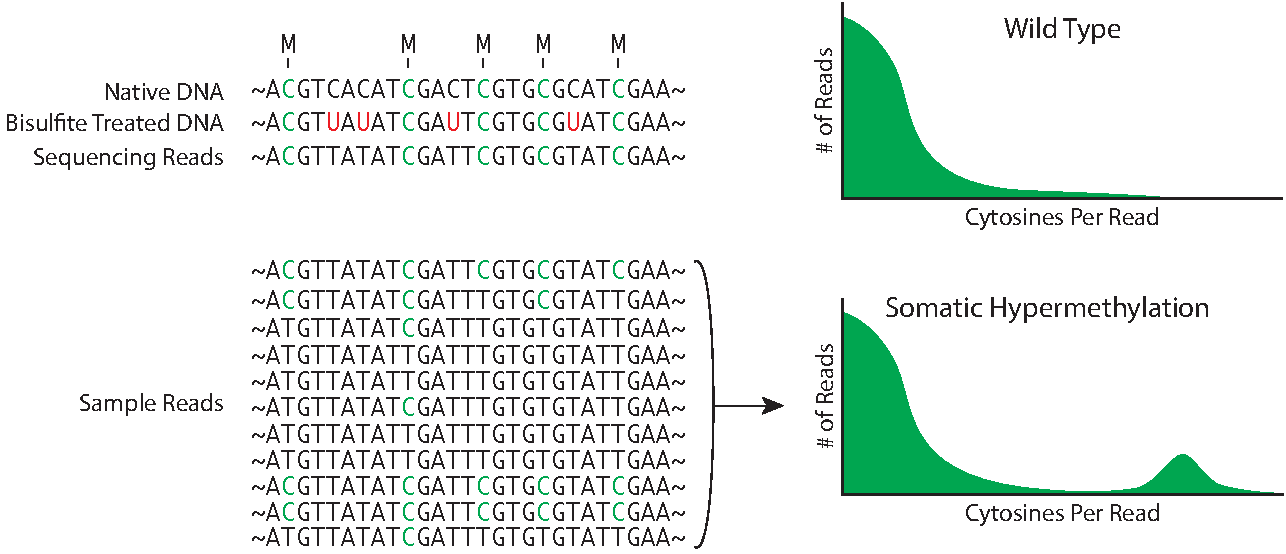
\includegraphics[width=5.8in]{Somatic_Hypermethylation}
\end{center}
\caption[Predicted Somatic Hypermethylation Profile]{\textbf{Predicted Somatic Hypermethylation Profile.} \\ Bisulfite treatment converts any unmethylated cytosines to uracil which is read as a thymine on the sequencing. Wild type DNA should have low levels of methylation and a long tail representing inefficiencies in the bisulfite conversion and sequencing errors (top right). In contrast, a sample with somatic hypermethylation should have a similar distribution to wild type DNA, but is expected to have a secondary peak representing reads with heavy methylation (bottom right).}
\label{Somatic_Hypermethylation}
\end{figure}
%%%%%%%%%%%%%%
I first identified CpG islands in the promoters of \italicize{ENG}, \italicize{ACVRL1}, and \italicize{SMAD4} (Figure~\ref{HHT_Promoters}) and designed primers to target the islands in \italicize{ENG} and \italicize{ACVRL1} (Figure~\ref{HHT_Primers}). Though \italicize{SMAD4} causes HHT, we did not design primers for this gene as we did not have any telangiectasia from individuals with a \italicize{SMAD4} germline mutation.
%%%%%%%%%%%%%%%
\begin{figure}[tbp!]
\begin{center}
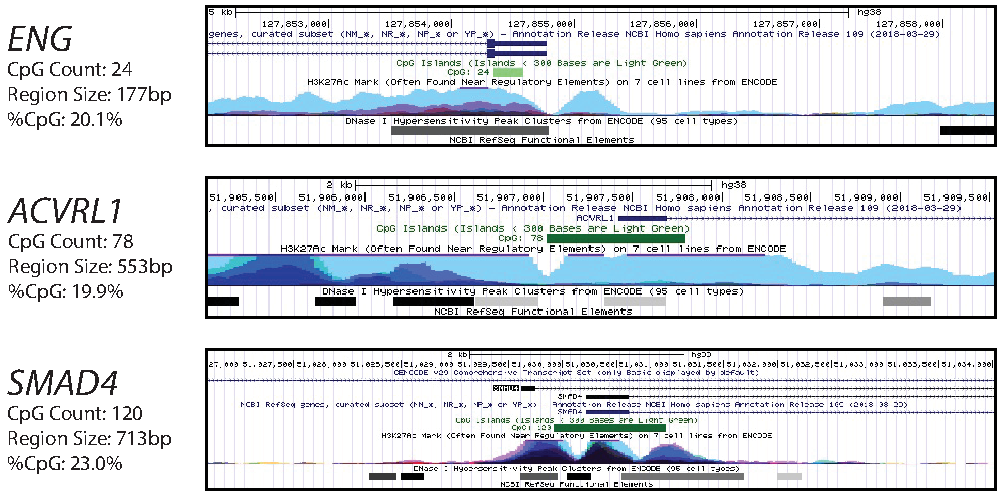
\includegraphics[width=5.8in]{HHT_Promoters}
\end{center}
\caption[CpG Islands in HHT Gene Promoters]{\textbf{CpG Islands in HHT Gene Promoters.} \\ UCSC genome browser images of the promoter regions of \italicize{ENG}, \italicize{ACVRL1}, and \italicize{SMAD4}. CpG islands are marked in light green. ($<$300bp) or dark green ($>$300bp) along with H3K27Ac marks over the region.}
\label{HHT_Promoters}
\end{figure}
%%%%%%%%%%%%%%
%%%%%%%%%%%%%%%
\begin{figure}[tbp!]
\begin{center}
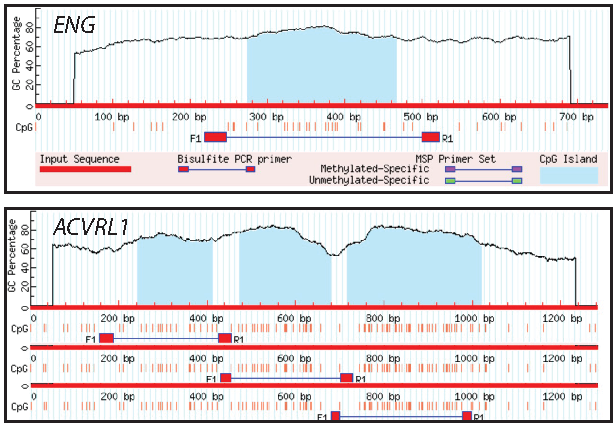
\includegraphics[width=5in]{HHT_Primers}
\end{center}
\caption[Primers Targeting CpG Islands in \italicize{ENG} and \italicize{ACVRL1}]{\textbf{Primers Targeting CpG Islands in \italicize{ENG} and \italicize{ACVRL1}.} \\ Primer design targeting dense regions of CpG dinucleotides (light blue) in \italicize{ENG} and \italicize{ACVRL1}. The CpG island in \italicize{ACVRL1} was too large to cover in a single amplicon, therefore I designed three primers to cover the regions of highest density, while designing primers to avoid CpGs which may impact annealing efficiency. }
\label{HHT_Primers}
\end{figure}
%%%%%%%%%%%%%%
As a control for these experiments we considered telangiectasia with a known somatic mutation as a negative control for somatic hypermethylation and compared them to mutation-negative telangiectasia which may have somatic hypermethylation as a means of LOF.

These experiments were ultimately uninformative as we observed high variability in the methylation rate in the \italicize{ENG} promoter and we only had a single sample with a germline mutation in \italicize{ACVRL1} that did not have a known somatic mutation (Figure~\ref{Methylation_Results}). 
%%%%%%%%%%%%%%%
\begin{figure}[tbp!]
\begin{center}
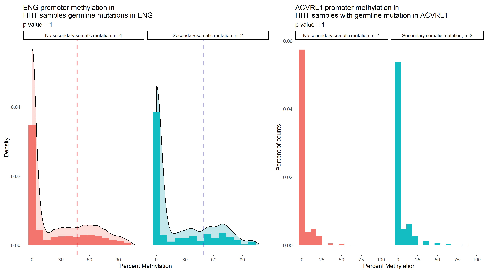
\includegraphics[width=5.8in]{Methylation_Results}
\end{center}
\caption[Promoter Methylation in \italicize{ENG} and \italicize{ACVRL1}]{\textbf{Promoter Methylation in \italicize{ENG} and \italicize{ACVRL1}.} \\  Methylation of telangiectasia with (green) or without (red) a previously identified somatic mutation for \italicize{ENG} (left) or \italicize{ACVRL1} (right). The \italicize{ENG} promoter shows high levels of somatic methylation in both the experimental samples and the controls. The \italicize{ACVRL1} promoter shows rather low level of basal methylation, but shows no significant secondary peak as might be expected by somatic hypermethylation.}
\label{Methylation_Results}
\end{figure}
%%%%%%%%%%%%%%
These results are likely confounded by the limited efficiency of bisulfite conversion as well a very limited sample size. In addition any somatic hypermethylation would be expected to occur mainly in endothelial cells; however, these crude punch biopsies contain a substantial amount of unaffected tissue around the telangiectasia, and endothelial cells are likely only a fraction of all cells in the biopsy. More samples will be required to determine if somatic hypermethylation of endothelial cells could result in LOF via silencing, though we will also need to overcome the technical limitations we encountered in these pilot experiments. 

Firstly, bisulfite conversion is not 100\% efficient. This is not a concern when evaluating germline methylation levels, however high conversion efficiency will be required to pick up low frequency somatic events in a highly heterogeneous tissue. As an alternative to bisulfite conversion, several long-read sequencing technologies (e.g. Pacbio and Oxford Nanopore) are capable of detecting DNA base modifications such as methylation during sequencing. This would be a more direct measure of methylation and would bypass the need for bisulfite conversion.

The second major limitation in these experiments is the heterogeneous tissue. It would be very beneficial to isolate endothelial cells prior to DNA extraction to increase the allele frequency of any potential somatic event. Traditionally this would be done by generating a single-cell suspension and staining for an endothelial cell-specific protein such as PECAM and sorting based on that marker. As we receive telangiectasia primarily from Canada, it is necessary that they be frozen prior to shipment which disrupts the cell membrane thereby precluding the generation of a single-cell suspension. However, I have had some success generating single-\italicize{nucleus} suspensions from telangiectasia, similar to what I have done for CCMs in Chapters 3 and 4. The nuclei yield from telangiectasia is low relative to CCMs (around 20,000 per telangiectasia), however it is feasible to stain these nuclei. The common endothelial cell stain PECAM is not present on the nuclear membrane; however the transcription factor ERG is present inside nuclei, and is highly specific to endothelial cells. ERG is a commonly used stain and I have attempted to stain nuclei with it, however my initial experiments were unsuccessful and I eventually abandoned the project in favor of bulk sequencing. This would be a powerful tool if a robust staining protocol could be developed. 

\subsection{Somatic Loss of Heterozygosity}
The second type of event I will discuss is somatic loss of heterozygosity (LOH) events. LOH is a general term that refers to loss of an allele resulting in a previously heterozygous site becoming homozygous. For example, loss of the wild type \italicize{ENG} allele in an individual with a germline \italicize{ENG} mutation would result in biallelic LOF and could theoretically be a source of the missing mutations. LOH can result from a variety of different genomic events such as a large deletion or mitotic recombination. Like somatic hypermethylation, LOH is a common mechanism in cancers to disrupt tumor suppressor genes. While targeted short-read sequencing is great for detecting small variants, it is blind to these chromosome-scale events which occur in a small number of somatic cells---i.e. we miss the forest for the trees. 

LOH in cancer samples is often detected via a SNP array such that an LOH event of reasonable frequency (often $\geq$25\%) can be visualized as a shift in copy number for a subset of markers---e.g. heterozygous markers in an unaffected region of the chromosome are present at 1~:~1 ratio, whereas markers over an LOH event at 25\% AF are present at a 1.25~:~0.75 ratio. This method works well for events with high allele frequencies, however the somatic variants I find in CCM and HHT are far lower, with most $<$5\%. This makes detection by SNP array challenging as we must identify a ratio of 1.05~:~0.95 in a fairly noisy assay. Reaching statistical significance with such a minor shift would require a dense SNP array and a large LOH event making this methodology infeasible. 

While detecting these events is nigh impossible with bulk sequencing, it is theoretically trivial with single-nucleus DNA sequencing (snDNA-seq). As an initial experiment, I performed snDNA-seq on familial CCM samples for which I did not find a somatic mutation. To detect somatic LOH in these samples, I needed only to sequence the pathogenic germline mutation and determine whether that heterozygous mutation was homozygous in some of the cells (Figure~\ref{Single_Cell_LOH}).
%%%%%%%%%%%%%%%
\begin{figure}[tbp!]
\begin{center}
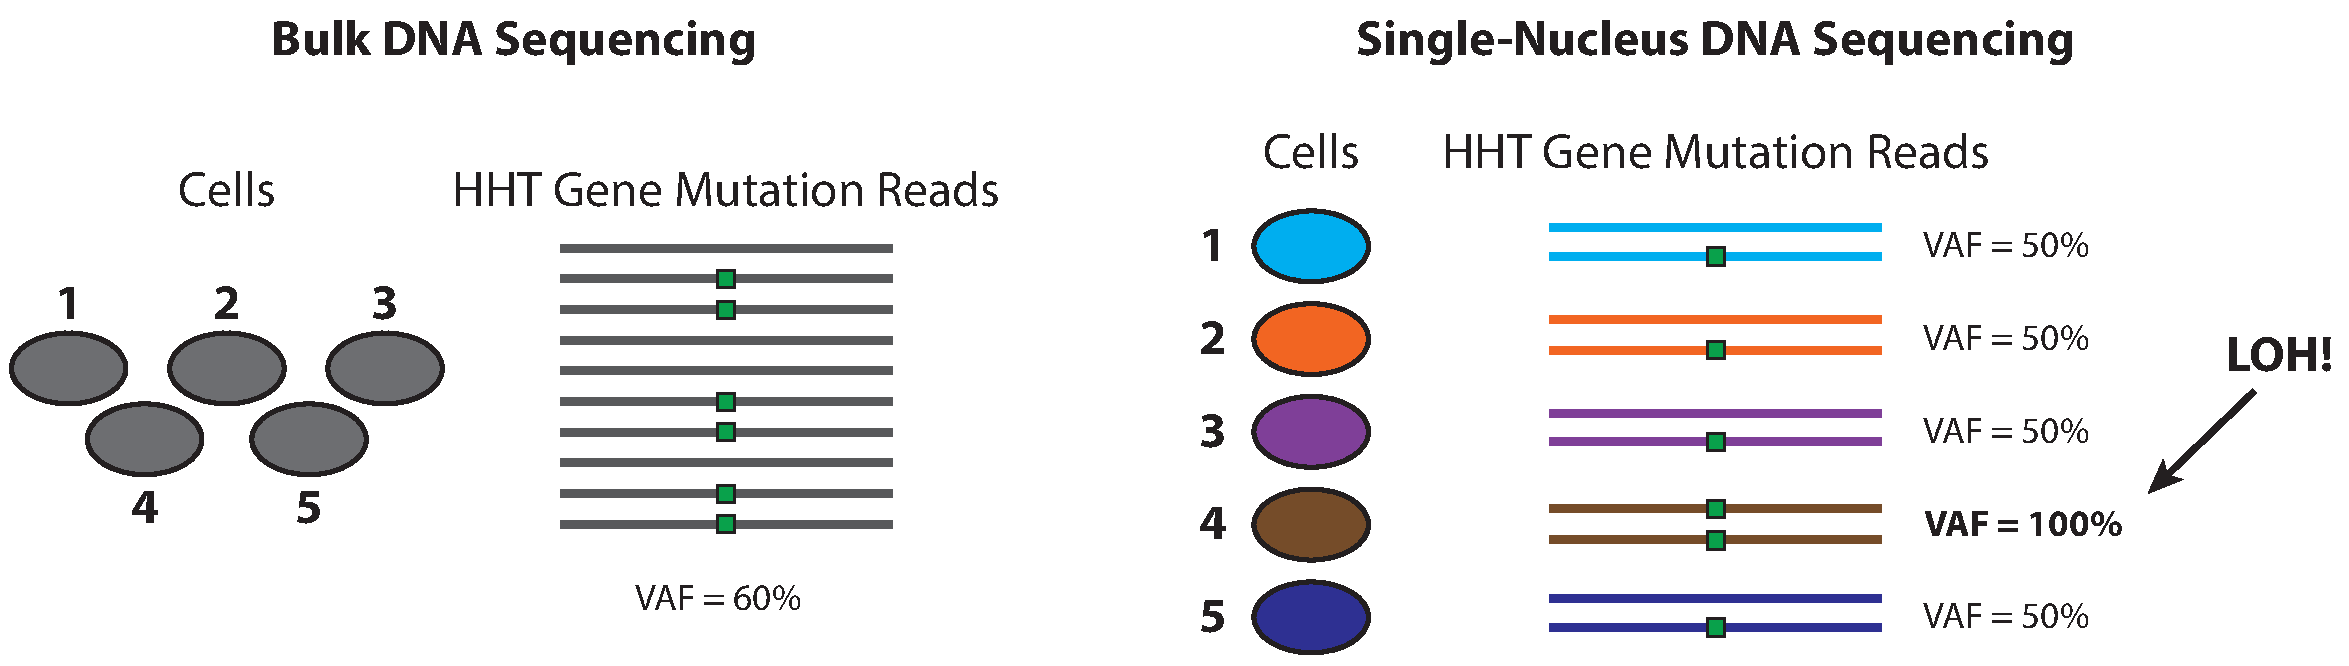
\includegraphics[width=5.8in]{Single_Cell_LOH}
\end{center}
\caption[Somatic LOH Detection with snDNA-seq]{\textbf{Somatic LOH Detection with snDNA-seq.} \\  Reads from bulk sequencing show a pathogenic mutation at an allele frequency of 60\%. From in reads from single-nucleus sequencing it is clear that four cells have the expected heterozygous genotype, but one cell is homozygous for the pathogenic mutation, indication a somatic LOH event. }
\label{Single_Cell_LOH}
\end{figure}
%%%%%%%%%%%%%%
The problem with this approach, as discussed in Chapter 3, is that snDNA-seq is confounded by stochastic allelic dropout (ADO) at a rate of 5--10\% per allele. As a result, if 1000 nuclei are sequenced, we find that around 800 have the expected heterozygous genotype, 100 will be homozygous for the reference allele, and 100 will be homozygous for the alternate allele. As ADO often occurs at similar or higher frequencies than the expected somatic LOH events, this targeted method is infeasible. 

In an attempt to overcome ADO I designed a panel for snDNA-seq that targets common SNPs such that we capture a high density of SNPs in the region of the genes of interest, with progressively lower density of markers towards the distal ends of the chromosome. This pattern was selected because there is a limit to how many markers we can use on a single panel (about 400 amplicons) and this pattern maximizes our chance of finding informative heterozygous SNPs in the region of the gene, while still maintaining some sensitivity for larger events that may impact a large portion of the chromosome. Any LOH event should convert multiple contiguous heterozygous markers to homozygosity and would theoretically be robust against random ADO of individual amplicons. Using this method, I again found that ADO was a major confounder. I initially expected that ADO would be largely stochastic such that each marker would be independent of the state of other markers. However, I found that ADO events were in fact `linked', such that a set of markers that was physically close on one allele would drop out as a set (Figure~\ref{Linked_ADO}). 
%%%%%%%%%%%%%%%
\begin{figure}[tbp!]
\begin{center}
\includegraphics[width=5.8in]{Linked_ADO}
\end{center}
\caption[Linked Allelic Dropout]{\textbf{Linked Allelic Dropout.} \\  Results of snDNA-seq of four SNPs, not involved in disease pathogenesis, that span a 50kb region and are all heterozygous in the germline. 85\% of the sequenced nuclei have the expected heterozygous genotype (Clone 1). However, Clones 2 and 3 show linked dropout of the entire alternate or reference allele at 6.3\% and 5.3\% respectively. Similarly, Clones 4 and 5 show linked dropout of the alternate allele in a smaller region of the last 2 or first 2 variants that are physically close.}
\label{Linked_ADO}
\end{figure}
%%%%%%%%%%%%%%
In effect, I was seeing dropout of entire haplotypes rather than individual markers. This likely reflects the mechanism by which ADO occurs. Mostly likely ADO results from incomplete lysis of nuclei which leaves some regions of chromosomes tightly bound in chromatin and inaccessible to primers. As the chromatin would be bound over a contiguous genomic region, we therefore get dropout of all markers that fall within the region of undigested chromatin.  This phenomenon unfortunately looks almost exactly like what we would expect to see from a genuine somatic LOH event, however there are some important differences that I attempted to leverage to discriminate between linked ADO and LOH. 

One critical difference between linked ADO and LOH is that linked ADO appears to occur randomly throughout the genome such that each nuclei should have a unique set of linked ADO products. In contrast, a biological LOH event should have identical breakpoints (Figure~\ref{LOH_ADO_Breakpoints}). 
%%%%%%%%%%%%%%%
\begin{figure}[tbp!]
\begin{center}
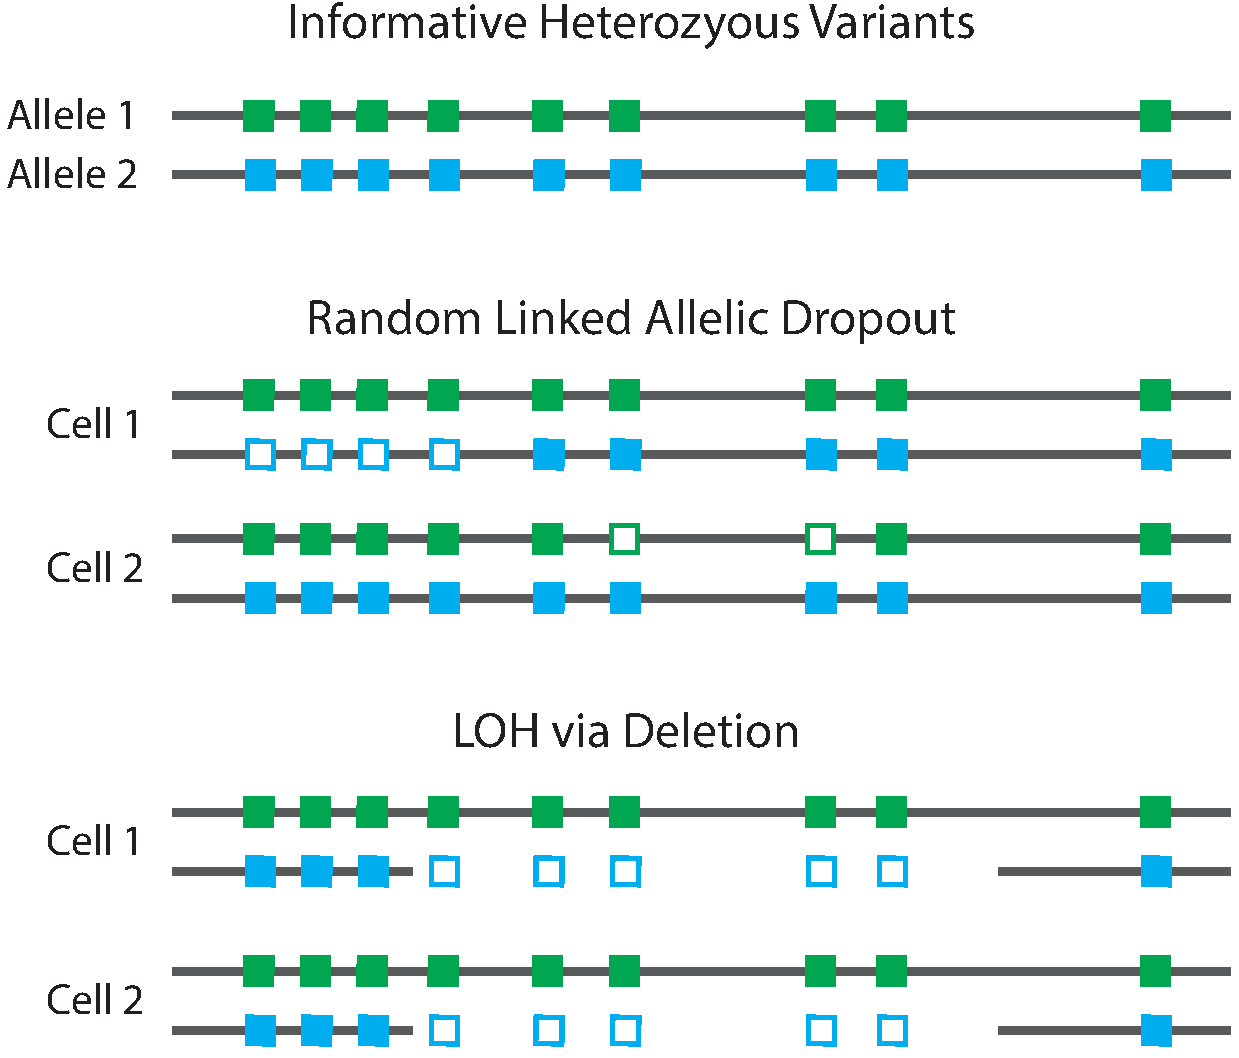
\includegraphics[width=4in]{LOH_ADO_Breakpoints}
\end{center}
\caption[Differences Between Linked ADO and LOH]{\textbf{Differences Between Linked ADO and LOH.} \\ Schematic illustrating differences between linked ADO and LOH by observing their effects on informative heterozygous variants on two alleles (green and blue squares). Linked ADO occurs randomly and affects both alleles equally as shown by dropped alleles (outlined squares). In contrast, LOH (caused by a deletion in this example) has identical breakpoints in all cells and is only present on a single allele. }
\label{LOH_ADO_Breakpoints}
\end{figure}
%%%%%%%%%%%%%%
The breakpoints generated by linked ADO and LOH can be determined in individual nuclei by identifying runs of homozygosity which can then be used to identify cells with identical breakpoints (My programs for this are available at \url{https://github.com/dasnellings/weaver}). In addition to differences in the breakpoints, linked ADO is expected to affect both alleles symmetrically, whereas LOH is asymmetric affecting only one allele.

In addition to leveraging the differences between linked ADO and LOH I have used one additional strategy to detect LOH events. Linked ADO occurs at a rate of 5--10\% and LOH events are expected to occur as a similar or lower frequency, however pathogenic LOH events are expected to result in biallelic LOF. In a sample where one somatic mutation is already known, we expect that the LOH event should be present in the same population of cells. Therefore, by excluding any cells that do not contain the known somatic mutation, we can effectively enrich for cells likely to have an LOH event and thereby increase the allele frequency of the LOH event above the ADO signal in this restricted population (Figure~\ref{LOH_Mutation_Strategy}). 
%%%%%%%%%%%%%%%
\begin{figure}[tbp!]
\begin{center}
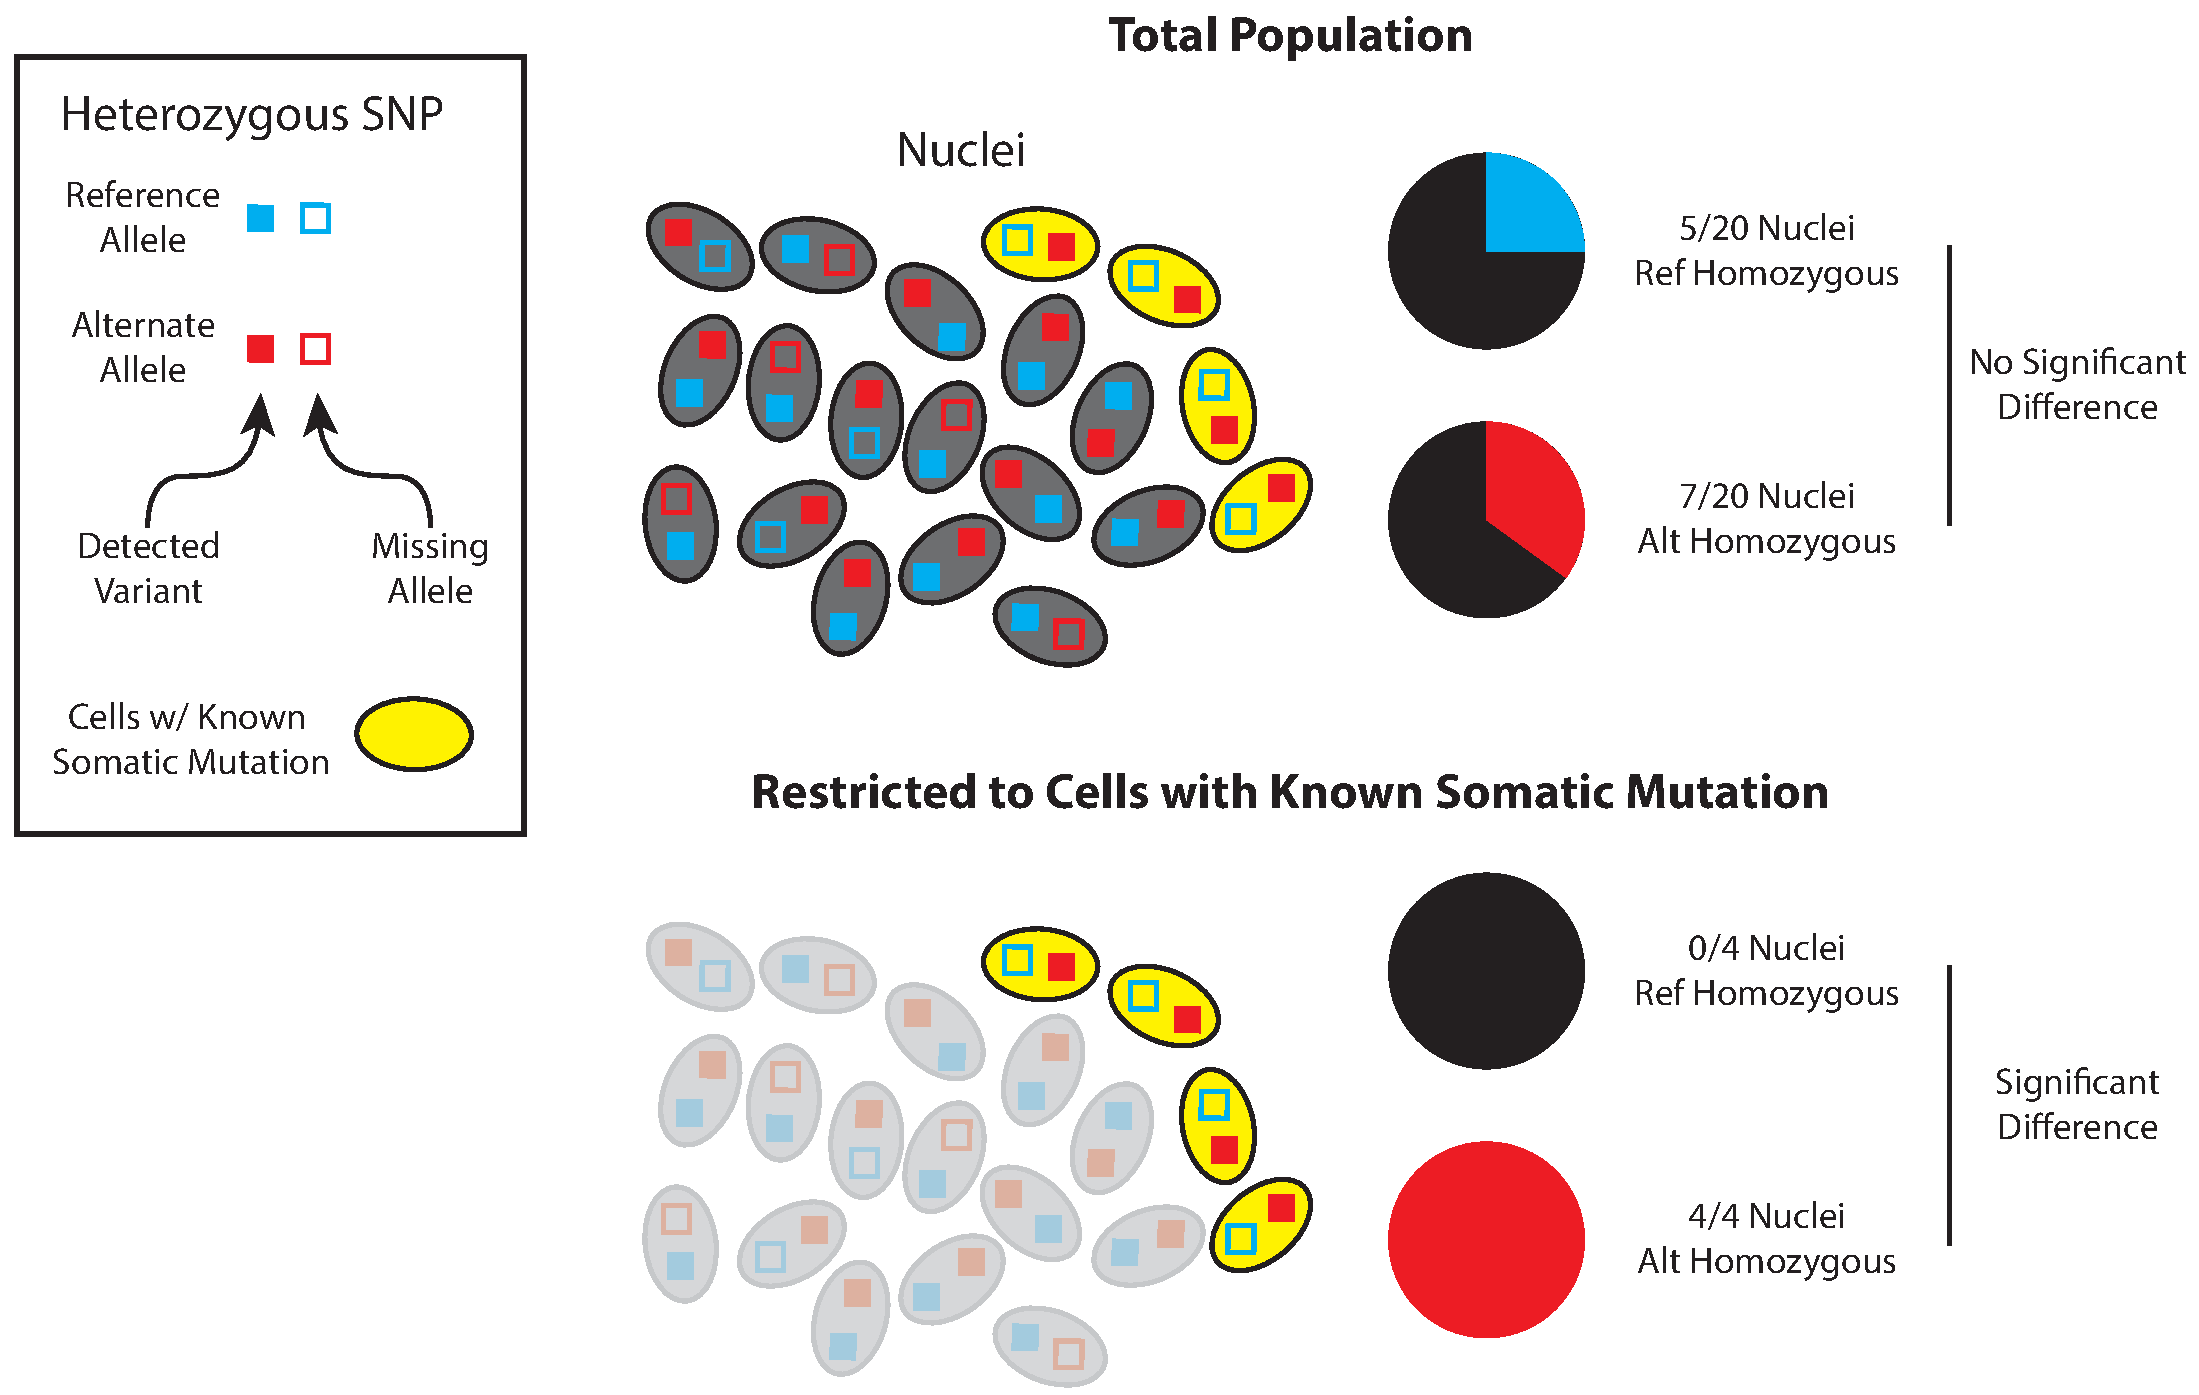
\includegraphics[width=5.8in]{LOH_Mutation_Strategy}
\end{center}
\caption[Leveraging Known Somatic Mutation for LOH Detection]{\textbf{Leveraging Known Somatic Mutation for LOH Detection.} \\  A known somatic mutation allows for enrichment of cells likely to have an LOH event. When considering the total population, the high rate of ADO confounds the detection of LOH events that occur at a similar frequency. However, when cells without a known somatic mutation are excluded, the LOH event may be enriched, increasing the allele frequency above the level of ADO noise.  }
\label{LOH_Mutation_Strategy}
\end{figure}
%%%%%%%%%%%%%%
The major limitation of this method is that it is only possible with samples that have at least 1 known somatic mutation, making it unusable for HHT and restricted to a subset of CCMs. 

I have used this panel design and analysis method on 15 CCMs, 10 of which had at least 1 somatic mutation that could be used to restrict the population. From these experiments, I have not identified any somatic LOH events that are likely to be pathogenic; however, in one sample I have identified a putative somatic LOH event on chromosome 12 that does not overlap \italicize{KRIT1}, \italicize{CCM2}, or \italicize{PDCD10} (Figure~\ref{Putative_LOH}). 
%%%%%%%%%%%%%%%
\begin{figure}[tbp!]
\begin{center}
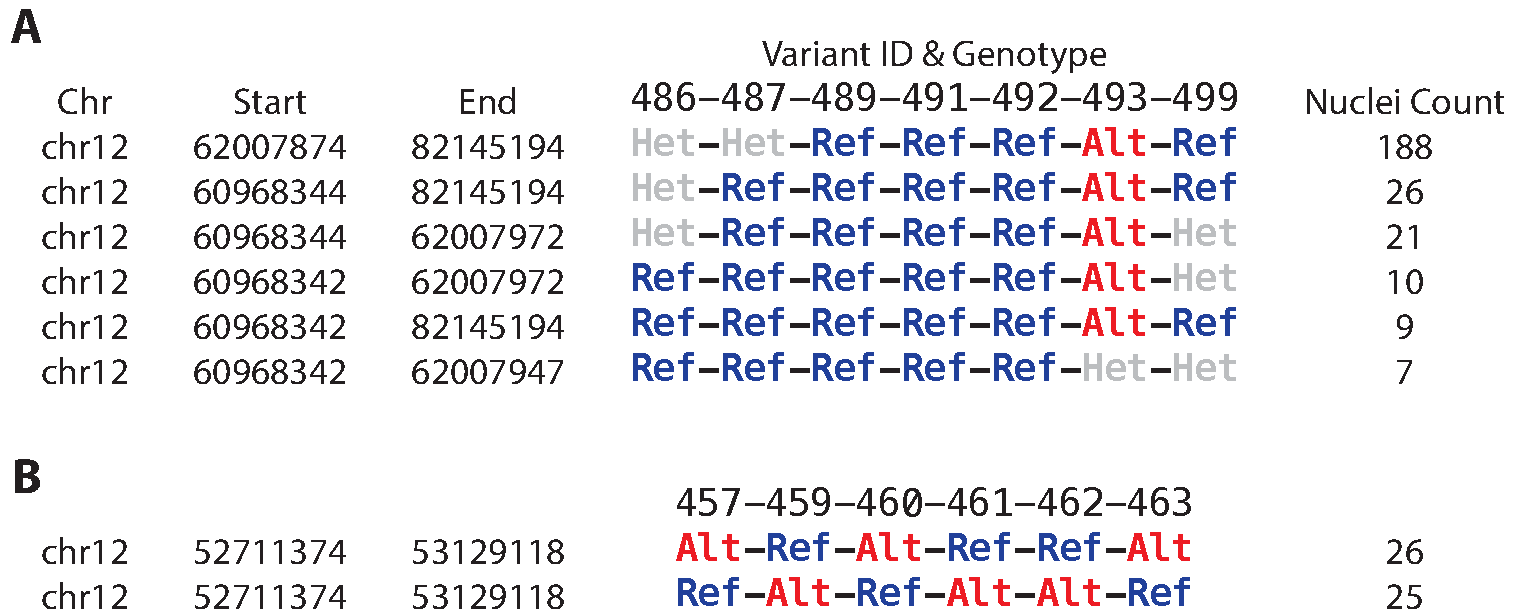
\includegraphics[width=5.8in]{Putative_LOH}
\end{center}
\caption[Putative Somatic LOH Event in a CCM]{\textbf{Putative Somatic LOH Event in a CCM.} \\ Runs of homozygosity present in CCM 5056 derived from snDNA-seq data from 2500 nuclei. \textbf{A}, 6 different runs spanning a 21Mb region. All 6 runs are likely generated from the same LOH event, however ADO on the edges of the event are likely generating false breakpoints. Note that there were no run of homozygosity for the reciprocal allele that consisted of at least 5 contiguous variants (the threshold for this analysis). \textbf{B}, An example of linked ADO from the same sample and chromosome showing symmetric dropout of both haplotypes at similar frequencies.}
\label{Putative_LOH}
\end{figure}
%%%%%%%%%%%%%%
This event is most likely an incidental finding, however this event should be confirmed by a secondary method as a validation of the methodology.

It is a near certainty that somatic LOH events may drive the formation of CCMs and telangiectasia in HHT, however their detection has thus far been elusive. It is currently unclear if this is due to the rarity of such events or if there remain flaws in my methodology that preclude their detection.







\section{Connection Between Sporadic Brain AVMs and HHT}
Brain AVMs are common in individuals with HHT, however the majority of brain AVMs in the population occur sporadically in individuals with no known genetic predisposition. This paradigm of similar pathologies in sporadic lesions and lesions from a familial genetic disorder is very similar to CCM. CCMs also have a familial and sporadic form and research from myself and others has shown that both forms share many aspects of pathogenesis and are ultimately caused by identical mutations. I hypothesized that this was also the case for sporadic and HHT-associated brain AVMs.

In Chapter 2 I showed that HHT-associated telangiectasia are caused by a two-hit mechanism. This study focused on telangiectasia as HHT-associated visceral AVMs are difficult to study since they are rarely resected in favor of embolization and radiosurgery. Unlike brain AVMs in HHT, sporadic brain AVMs are commonly resected and are readily available to researchers. Previous studies found that many sporadic brain AVMs have a somatic mutation in \italicize{KRAS} \citep{nikolaev2018}, however it remains unclear if these samples may have additional mutations. To test whether sporadic brain AVMs harbor somatic mutations in \italicize{ENG}, \italicize{ACVRL1}, or \italicize{SMAD4}, I sequenced 68 presumed sporadic brain AVMs that were surgically resected at the Barrow Neurological Institute. 

As reported by others I found that 24 of the 68 had a gain of function mutation in \italicize{KRAS}. I also identified one sample with a gain of function mutation in \italicize{TEK} (p.L194F) which is known to cause venous malformations \citep{limaye2009}. This sample may represent a novel mutation for AVMs, but more likely is the result of a misclassification of a venous malformation as an AVM. One additional sample has a mutation in \italicize{VHL} (p.N78S) which has been shown to be moderately activating in some assays \citep{rechsteiner2011}, however it remains unclear if this is a causal mutation for AVMs. In one sample I found a germline missense mutation in \italicize{ENG} (p.R406C, 550/1178 reads, 47\% VAF) which has not been previously reported to cause HHT, however given the context, it is highly likely to be pathogenic. I reviewed the case notes from the Barrow Neurological Institute for this individual and there was no information that could either support or reject an HHT diagnosis (telangiectasia, family history, epistaxis). Notably, this sample did not have a GOF mutation \italicize{KRAS} and I did not identify any somatic mutations in \italicize{ENG}. 

In 3 of the 68 brain AVM samples I found a mutation in \italicize{ASXL1} (p.S1344F, p.W591*, p.Q512*), the latter found in a sample with a GOF \italicize{KRAS} mutation. These mutations are all likely to cause LOF. LOF mutations in \italicize{ASXL1} have never been reported in a vascular malformation, however they are commonly found in cases of clonal hematopoiesis---a phenomenon where hematopoietic stem cells responsible for forming blood cells acquire mutations that give them a survival advantage and become the dominant clone in the blood as an individual ages \citep{fujino2020}. This finding was initially very exciting as the mutation was found in multiple brain AVM samples; however, upon reevaluation it is most likely that these individuals had some degree of clonal hematopoiesis and we picked up the \italicize{ASXL1} mutation from residual blood present in the AVM sample. I encountered a similar issue in an HHT-associated pulmonary AVM where I identified a well-studied GOF mutation in \italicize{DNMT3A} (p.R882H, 57/1029 reads, 5.5\% VAF). Similar to \italicize{ASXL1}, mutations in \italicize{DNMT3A} have not been reported in vascular malformations, but they are common in cases of clonal hematopoiesis \citep{buscarlet2017}. This finding suggests mutations in blood cells could be a major confounder when searching for mutation in vascular malformations, and highlights the importance of paired blood sequencing.

These initial data suggest that while HHT-associated brain AVMs and sporadic brain AVMs have similar pathologies, they are genetically distinct. However, additional studies---especially of HHT-associated AVMs---will be required to fully understand their genetic underpinnings. 







\section{Syndromic Brain AVMs in the Amish}
In 1997, members of the Marchuk lab collected blood samples from a large 12-generation kindred of the Amish of Lancaster Pennsylvania who develop syndromic brain AVMs. This kindred includes 6 individuals (2 female, 4 male, none are first-degree relatives) with a confirmed AVM in the brain or spinal cord; however, only 5 were available for sample collection. As the Amish are a small insular community, it is possible that this AVM syndrome is caused by a rare ancestral mutation that has reached autozygosity in the affected individuals. As the Amish of Lancaster keep meticulous genealogical records, previous members of the lab were able to determine that the 6 affected individuals were born from pairings with kinship coefficients between 0.009 and 0.032. The inheritance pattern strongly suggests autosomal recessive inheritance; however, as with other genetic VM disorders it is likely that there is reduced penetrance. During sample collection, individuals filled out a survey with symptoms and several of the `unaffected' individuals reported seizures and frequent headaches which are common symptoms of brain AVMs. As the Amish eschew health insurance, the only MRI available for these individuals are of low quality and were ultimately inconclusive. 

Several previous members of the Marchuk lab have attempted to find the causal mutations in this kindred and there have been several mapping studies performed using SNP arrays. These mapping efforts revealed several putative regions of autozygosity on chromosomes 9 and 15 that were promising candidates, though a causal mutation was not found. To follow up on these previous efforts, I performed whole-exome sequencing on 4 of the affected individuals and whole-genome sequencing on 1 affected individual to validate the previously mapped regions of autozygosity and to identify a pathogenic variant. Due to the reduced penetrance, I only sequenced affected individuals as it was not possible to determine who is not affected. From these analyses, I determined 9 regions of autozygosity shared between all 5 individuals across chromosomes 2, 3, 11, 14, 19, and 20 (Figure~\ref{Amish_Autozygosity}).
%%%%%%%%%%%%%%%
\begin{figure}[tbp!]
\begin{center}
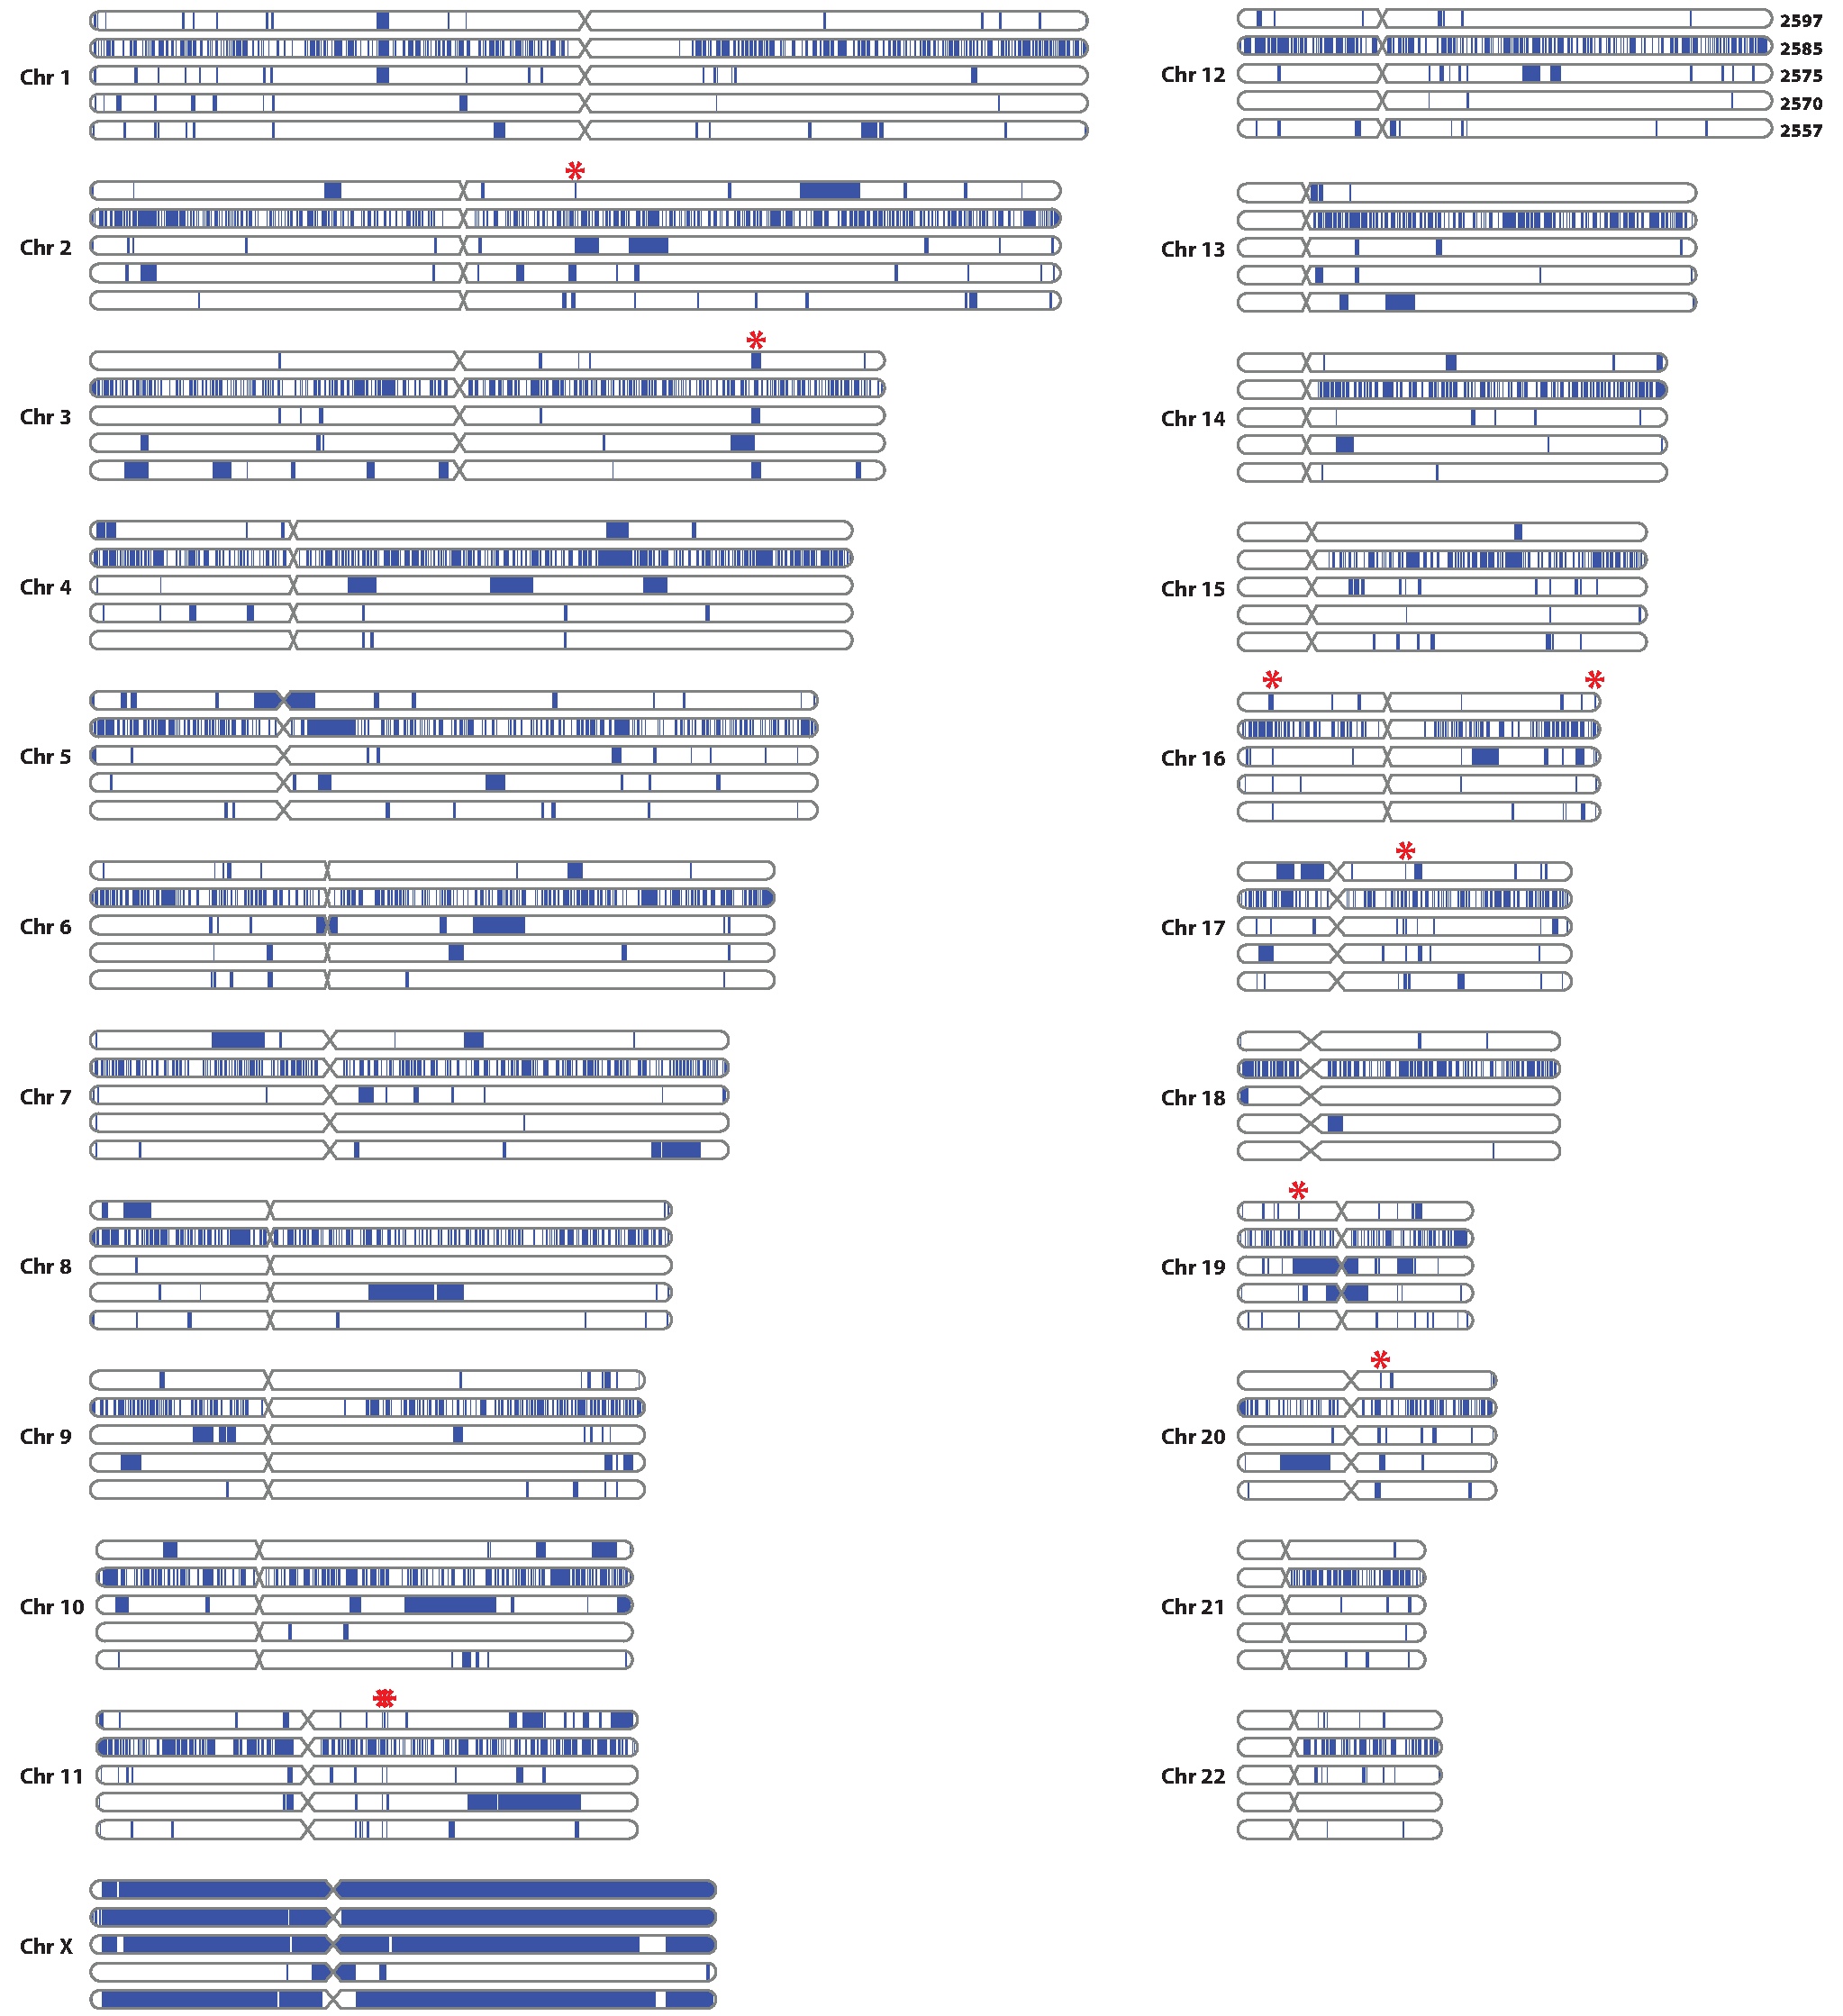
\includegraphics[width=5.9in]{Amish_Autozygosity}
\end{center}
\caption[Autozygosity in Amish with Syndromic Brain AVMs]{\textbf{Autozygosity in Amish with Syndromic Brain AVMs.} \\ Regions of presumed autozygosity (blue bars) in the autosomes and ChrX in 5 individuals with syndromic brain AVMs. The red * shows regions of autozygosity that are present in all 5 individuals. Note that the data from sample 2585 is derived from whole-genome sequencing data and therefore has finer resolution than the other samples which are derived from whole-exome sequencing data. Samples 2597, 2585, 2575 and 2557 are from males and are presumed to be hemizygous across ChrX. Sites on ChrX that were determined to be heterozygous in these samples are likely the result of either sequencing errors or misalignments.}
\label{Amish_Autozygosity}
\end{figure}
%%%%%%%%%%%%%%
 Notably, none of the previously identified regions were validated. I manually examined the previously determined regions on chromosomes 9 and 15 and found that, while the markers used in the initial study were accurate, there were heterozygous variants in between markers that disrupted the putative regions of autozygosity. 

I did not identify any putative pathogenic variants within the regions of autozygosity that I identified. I also identified regions that were autozygous in only 4 of the 5 individuals and again failed to find any putative pathogenic variants in these regions. I broadened my search to no longer be restricted by regions of autozygosity, and again failed to find any likely pathogenic homozygous variants in these individuals. I also manually examined variants in the previously identified regions on chromosomes 9 and 15 and failed to find any likely pathogenic homozygous variants. To explore the possibility that there were two different variants in the same gene, I expanded my search to heterozygous variants, present at $<$1\% population allele frequency in gnomAD, and filtered for nonsynonymous variants. I did not find any recurrently mutated genes shared between these individuals. Note that I did not find any mutations in \italicize{ENG}, \italicize{ACVRL1}, or \italicize{SMAD4}.

The variants I identified to this point have been single nucleotide variants, small insertions, or small deletions. These variants are readily detectable with traditional variant callers, however these variant callers are not able to detect structural variation. Calling structural variants from exome sequencing data is challenging due to sparse coverage, however I was able to identify structural variants in sample 2585 for which I performed whole-genome sequencing. This analysis was performed with Manta using whole-genome sequencing data from blood outgrowth endothelial cells from an individual with HHT as a negative control \citep{chen2016}. From this analysis I identified 601 putative structural variants that were homozygous in sample 2585 and absent in the negative control. Resources for programmatic adjudication of structural variants are sparse, specifically aggregate population allele frequency data, therefore I manually analyzed each putative variant while discarding any putative variant that was present in the NCBI Curated Common Structural Variants study (NCBI study accession no: nstd186) or the Database of Genomic Variants \citep{macdonald2014}. The majority of putative variants were either of poor quality or were present in the aforementioned databases; even so, there remain many high quality, undocumented variants. Several of the remaining variants fall in regions that overlap known ENCODE elements, the boundaries of topologically associated domains, and non-coding RNAs, however the impact of these variants remains unclear. Future studies should focus on performing whole-genome sequencing of additional samples to narrow the list of putative variants, and perform functional validation of any promising candidates. 







\section{Mosaicism in CCM}
% BaseScope



\section{Sturge-Weber Syndrome and Somatic Mutations in \italicize{GNAQ}}
Surge-Weber syndrome (SWS) is a sporadic vascular disease characterized by a mosaic capillary malformation (aka port-wine stain) present at birth and a leptomeningeal angioma in the brain. Unlike CCM and HHT, SWS is an exclusively sporadic disease, with no heritable component. A genetic study of SWS found that the capillary malformation and the leptomeningeal angioma are caused by a somatic GOF mutation in \italicize{GNAQ} \citep{shirley2013}. Notably, this study also found that facial capillary malformations not associated with SWS are caused by the same mutation. The observation that SWS is due to a genetic mutation, yet is not heritable, suggests that GOF in \italicize{GNAQ} would not be viable when transmitted through the germline, and therefore SWS can only exist when the mutation occurs during postzygotic development---as was predicted by Rudolf Happle \citep{happle1987}.

The genetics of \italicize{GNAQ} has captured my interest as it turns out that activating mutations are not only found in SWS, but also in uveal melanoma (a bona fide cancer) \citep{shoushtari2014}, and circumscribed choroidal hemangioma \citep{leguin2019}. I found it curious that activation of the same gene could lead to these disparate phenotypes. More interesting yet, these diseases all have highly specific and distinct \italicize{GNAQ} mutational spectra: SWS is dominated by p.R183Q (although we recently found 1 case of a non-SWS capillary malformation with p.Q209R), circumscribed choroidal hemangioma is highly specific for p.Q209R, whereas the vast majority of uveal melanomas have p.Q209L or p.Q209P with a minority having p.R183Q or p.Q209R. Based on this rigid genotype-phenotype correlation I hypothesized that---while all of these mutations activate \italicize{GNAQ}---they promote distinct modes of activation that result in different phenotypes. 

To test this hypothesis, Francesca Galeffi and I transfected human microvascular endothelial cells in culture with a plasmid containing 1 of 5 variants of \italicize{GNAQ}: wild type, p.C9X, p.R183Q, p.Q209R, or p.Q209L. We performed RNA-seq on these cultures in triplicate to determine if the different mutation in \italicize{GNAQ} were activating distinct transcriptional programs in endothelial cells. 

%\subsection{Happle's hypothesis}
%\subsection{\italicize{GNAQ} in uveal melanoma and circumscribed choroidal hemangioma}
%\subsection{Link between SWS, UM, and CCH?}








\section{Somatic Mutations in Infantile Hemangioma}
Infantile hemangioma (IH) are one of the most common vascular malformations. They occur in children and are typically present at birth as a red spot flush with the surrounding skin. Soon after birth the hemangioma rapidly grows and becomes raised from the skin. They are generally benign and are typically left alone unless they cover the child's mouth, nose, or eyes. What makes IH so interesting compared to other types of vascular malformations is that they almost always completely regress within the first few years of the child's life. While other types of vascular malformations may spontaneously regress (telangiectasia and AVMs), none do so with the consistency of IH. This phenomenon has been of great interest, not for the purpose of developing therapeutics for IH (propranolol is an extremely effective treatment for IH) but for uncovering the mechanism of regression in the hopes that what we learn can be applied to regress other, more nefarious, vascular malformations. 

\subsection{GLUT1 in IH endothelium}
Perhaps one of the most provocative discoveries into the mechanism of IH pathogenesis is the fact that endothelial cells from IHs highly express GLUT1 \citep{north2000, north2001}. GLUT1 is a glucose transporter that has remarkable specificity for the placental endothelium. This finding suggested that the IH may be comprised of cells that dislodged from the maternal placenta, then became hyper-proliferative in a post-fetal environment. If this hypothesis is correct, one would expect to find that the IH is a genetically chimeric growth between fetal and maternal cells. This hypothesis was put to the test using fluorescence \italicize{in situ} hybridization to assay the presence of XX cells in IH from a male infant with confirmation by sequencing microsatellites and SNPs that were divergent between mother and child. This analysis found no evidence for maternal-fetal chimerism in IH \citep{pittman2006}. Despite this counter-evidence, the presence of GLUT1 in IH is strongly indicative of some link with the placenta though unfortunately this link currently remains elusive. The current literature has very clearly shown the presence of GLUT1 in IH endothelial cells, however the extent of the placental transcriptional program is unclear. Epigenomic profiling of paired IH and maternal placental samples may give valuable insights into the mechanism of IH. 

\subsection{Efforts to find somatic mutations in IH}
As it is quickly becoming clear that the vast majority of vascular malformations are the result of somatic mutations---many occurring in known oncogenes---I thought that somatic mutations may also underlie IH. To test this, I sequenced 61 IH lesions on an 'oncopanel' covering many genes that are highly mutated in cancers as well as several genes previously implicated in vascular malformations (\italicize{KRIT1, CCM2, PDCD10, ACVRL1, ENG, SMAD4,} etc.) Unfortunately after filtering putative variants, no there were no variants with likely functional significance and that occurred in more than a single sample. I am aware of at least 1 other group that has attempted to identify somatic mutations in IH via whole-exome sequencing, however to date there are no known somatic mutations in IH. One important aspect of these studies that must be noted is that they are invariably focused on coding regions of the genome. Non-coding variants are more than capable of causing disease however discovery-focused sequencing studies often ignore non-coding regions both because of the cost of sequencing the entire genome to a depth sufficient to detect somatic mutations, and the challenges associated with functional analysis of non-coding variants. Further studies may find that somatic mutations do cause IH, but they occur in a region of the genome that is missed by the majority of sequencing studies. 









\section{CCM \& Meningioma}
Although the vascular lesions are the primary sequelae of familial CCM, many groups have noted an increased prevalence of meningioma in individuals with familial CCM---especially those with a mutation in \italicize{PDCD10} \citep{labauge2009, riant2013, garaci2015}. In addition, we have previously been contacted by an individual whose child had a sporadic CCM that regrew into a meningioma. Unfortunately we were unable to acquire a tissue sample for genetic analysis, however this case along with the strong link between familial CCM and meningioma has fueled my interest in understanding the link between CCM and meningioma. 

\subsection{Kruppel-like factor 4 (\italicize{KLF4})}
\italicize{KLF4} is a transcription factor with key roles in the pathogenesis of both CCM and meningioma. In CCM, \italicize{KLF4} (along with \italicize{KLF2}) is a key player in CCM signaling that is upregulated by loss of the CCM complex or gain of function in \italicize{MAP3K3} \citep{cuttano2016, zhou2016}. Indeed, overexpression of \italicize{KLF4} in mouse models leads to an aggressive CCM-like phenotype \citep{ren2021}. In meningioma, mutations in \italicize{KLF4} are common and often co-occur with mutations in \italicize{TRAF7} \citep{reuss2013}. In addition, \italicize{KLF4} mutated meningioma have been shown to be responsive to treatment with temsirolimus \citep{vonSpreckelsen2020}—a derivative of rapamycin (sirolimus) which has been shown to be effective in treating CCM in mice \citep{ren2021}. The importance of \italicize{KLF4} in both CCM and meningioma suggests that dysregulation of \italicize{KLF4} may underlie the development of meningioma in individuals with familial CCM. 

The majority of \italicize{KLF4} mutations found in the catalog of somatic mutations in cancer (COSMIC) result in p.K409Q (Figure~\ref{KLF4_COSMIC}A). This narrow spectrum of mutations suggests that the p.K409Q variant results in KLF4 gain of function. Notably, the p.K409Q mutation is highly specific to meningioma, occurring in very few other cancer types (Figure~\ref{KLF4_COSMIC}B). The KLF4 protein contains 3 DNA-binding zinc-finger domains that contribute to its activity as a transcription factor. The p.K409Q mutation occurs in the first of the three zinc-finger domains (Figure~\ref{KLF4_COSMIC}C). A structural study of KLF4 determined that the second two zinc-finger domains consistently bind DNA, however the first zinc-finger only sometimes participates in DNA binding \citep{schuetz2011}. They determined that the second and third domains are required for site specificity, but the third "inhibits cryptic self-renewal and block of differentiation activity". This immediately suggests a mechanism by which the p.K409Q mutation may disrupt the inhibitory capacity of KLF4 while retaining its functions that are independent of the first zinc-finger domain. 

%%%%%%%%%%%%%%%
\begin{figure}[tbp!]
\begin{center}
\includegraphics[width=5.8in]{KLF4_COSMIC}
\end{center}
\caption[\italicize{KLF4} Mutations in COSMIC]{\textbf{\italicize{KLF4} Mutations in COSMIC. } \\ \textbf{A}, Distribution of somatic mutations in \italicize{KLF4} that are present in the catalog of somatic mutations in cancer (COSMIC). The location of the most frequent mutation (p.K409Q) is expanded in the inset. \textbf{B}, Distribution of \italicize{KLF4} p.K409Q in tissue types present in COSMIC. C. Structure of KLF4 zinc-finger domains bound to DNA (PDB: 2WBU). Border box denotes the expanded region to the right showing the interaction between K409 and the DNA backbone.}
\label{KLF4_COSMIC}
\end{figure}
%%%%%%%%%%%%%%

I though that since overexpression of \italicize{KLF4} is sufficient to cause CCM in mice, the p.K409Q mutation may cause some sporadic CCMs in humans. To test this, I developed a ddPCR assay to test for this mutation in 30 mutation-negative sporadic CCM, however I did not find evidence for this mutation in any of these samples. This may be a reflection of the highly specific functions of the first zinc-finger domain in KLF4 as discussed above. This function may be critical for meningioma development, but less important for CCM development. However, the inverse is not necessarily true---i.e.~while the p.K409Q mutation may not cause CCMs, overexpression of \italicize{KLF4} may cause meningioma. This is currently unknown, though if true, may account for the presence of meningioma in familial CCM. One straightforward way to test this hypothesis would be to sequence tissue from meningioma in individuals with familial CCM. I suspect that these meningioma harbor a somatic loss of function mutation in \italicize{KRIT1/CCM2/PDCD10} leading to biallelic loss of a CCM gene resulting in upregulation of \italicize{KLF4}. These meningioma may also harbor a second mutation in \italicize{TRAF7} which have often been found in non-CCM meningioma. Unfortunately, tissue samples of meningioma from individuals with familial CCM have been difficult to acquire, thus I have been unable to test this hypothesis. However, I expect that future studies will find that \italicize{KLF4} is a critical link between CCM and meningioma. 



%\section{Genomic Instability in Vascular Malformations}



%\section{Cell Non-autonomous Effects in CCMs}



%\section{Single-Nucleus Phased Droplet Genotyping}
% SNuPDoG???





%\section{The Molecular Basis of Genetic Dominance}
%\subsection{Phenotypic Dominance $\neq$ Genetic Dominance}
%\subsection{Knudsons Fingerprint}
%\subsection{The Diverse Functional Effects of Genetic Mutations}










%\section{The Intersection of Somatic Mutagenesis and Evolution}
%\subsection{The Creation of New Alleles}
%\subsection{The Relationship Between Mutability and Fitness Landscape}
%\subsection{Recurring Mutations \& Convergent Evolution}
%\subsection{Clonal Evolution of Somatic Mutants}
%\subsection{Cancer}










%\section{Somatic Mutations}
%\subsection{The Role of Somatic Mutations in Aging}
%\subsection{Constitutional Intolerance \& Somatic Permissiveness}
%\subsection{Somatic Reversion of Pathogenic Mutations}
%\subsection{What is the Consequence of RNA Mutations?} 
%mutations at the RNA level i.e. individual mutant RNA molecules
%interactions with the ribosome?
%could a single RNA molecule screw things up?

